\section{Implementation}
\label{ch:impl}
\noindent	

\subsection{CoAP-server}
As mentioned in chapter \ref{ch:method:tech} the CoAP-server is implemented in Go using an external library \cite{goCOAP}. The library implements CoAP similarly to how Go normally handles HTTP. To start serving CoAP a router is created for routing request to different locations. A middleware was created to enable logging. The first rout added was the rout to get the mock temperature sensors. To create a rout an endpoint and a handler function needs to be provided to the router. In figure \ref{code:router} we can see the code snipped to create the router, add the middleware and lastly creating the first route.

\begin{figure}[H]
    \begin{lstlisting}[language=go]
r := mux.NewRouter()
r.Use(loggingMiddleware)
r.Handle("/temp", mux.HandlerFunc(handleTemp))
    \end{lstlisting}
    \caption{Go code snipped showing creating the CoAP router, adding a logging middleware and creating the handler for temperature}
    \label{code:router}
\end{figure}

The temperature handler decodes the incoming CoAP message to figure out what type of request it was. It also checks if the message has a payload. All the request types to this endpoint requires a payload. Figure \ref{code:temp:body} shows the code snippet for the initial handling of a request to the temperature endpoint. If the body does not exist it ends the request there by responding with bad request.
\begin{figure}[H]
    \begin{lstlisting}[language=go]
method := r.Code.String()
body := make([]byte, 128)
if r.Body == nil {
    w.SetResponse(codes.BadRequest, message.TextPlain, bytes.NewReader([]byte(string("No body included"))))
    return
}
n, _ := r.Body.Read(body)
body = body[:n]
\end{lstlisting}
    \caption{Code showing initial handling of the temperature request}
    \label{code:temp:body}
\end{figure}

The handler can handle 4 different request types: GET, POST, PUT, DELETE. 

GET responds with the current temperature of the processor if it exists otherwise it returns not found. Because the sensor is simulated, after the GET request it either increase or decrease the temperature of the sensor by a random amount between 1-3$^{\circ}C$. Figure \ref{code:temp:struct} shows the structure for a temperature sensor.

\begin{figure}[H]
    \begin{lstlisting}[language=go]
type TemperatureSensor struct {
    Status      bool
    Temperature int
    Location    string
}
\end{lstlisting}
    \caption{Structure for a mock temperature sensor}
    \label{code:temp:struct}
\end{figure}

POST creates a new temperature sensor. The request requires the payload to contain both the location of the sensor and the initial power status. When the request is received it creates a new instance of a temperature sensor. It assigns the values received and randomizes a temperature between -20-30$^{\circ}C$. If the request is successful it responded with status code created.

PUT request are used to switch power status. The request requires the body to contain the new power status and the name of the sensor to be changed. If the
sensor exists it changes its power status and responds with status Changed.

DELETE request removes a sensor if the payload includes the sensor name. If the request is successful it responds with Deleted.

For clients to be able to discover what temperature sensors is available the /all endpoint was created. This endpoint only accept GET request and uses Go's built in JSON library to convert the internal map of sensors to a JSON string to include in the response. The code implementation can be found in figure \ref{code:temp:all}.

\begin{figure}[H]
    \begin{lstlisting}[language=go]
r.Handle("/all", mux.HandlerFunc(func(w mux.ResponseWriter, r *mux.Message) {
    data, _ := json.Marshal(thermostats)
    w.SetResponse(codes.Content, message.TextPlain, bytes.NewReader(data))
}))
\end{lstlisting}
    \caption{Creation of the /all endpoint}
    \label{code:temp:all}
\end{figure}

The last endpoint is /pi which enables clients to gather information about the CoAP-server's processor and memory utilization. The server collects this data through the Linux proc files. CPU information is gathered through the proc/stat file while the memory is gathered through the proc/meminfo file. I used a library to help width parsing these files\cite{goProc}. A separate thread reads the proc files every second. For CPU usage it uses the last calculated value to derive the current usage in percentage. For the memory the proc/meminfo contains both free memory and total memory. From this the function derives the current usage in the format used/total.

\subsection{Translator}
The translator builds on a previous implemented CoAP client in Go. To translate from CoAP to MQTT a MQTT library was added to the project\cite{goMQTT}. The translator will poll data from the CoAP and then publish it to the MQTT-broker. It will also subscribe to certain MQTT messages to be able to convert them to CoAP request. The response from these messages will then be published.

The first thing the Translator does is send a request to the CoAP-server to retrieve the available sensor. This is to keep an internal map of what sensor are online to prevent the Translator to pull unnecessary data. After it retrieves the information about the temperature sensors it starts the connection to the MQTT broker and creates some constant subscriptions. When subscribing the MQTT library requires callback functions that will fire when a message is received to that topic. The connection code can be found in figure \ref{code:translator:connect}

\begin{figure}[H]
    \begin{lstlisting}[language=go]
populateSensors()
var broker = "localhost"
var port = 1883
opts := mqtt.NewClientOptions()
opts.AddBroker(fmt.Sprintf("tcp://%s:%d", broker, port))
opts.SetClientID("Coap Translator")

opts.SetDefaultPublishHandler(messagePubHandler)
opts.OnConnect = connectHandler
opts.OnConnectionLost = connectLostHandler
opts.SetPingTimeout(time.Second * 60)

client := mqtt.NewClient(opts)

if token := client.Connect(); token.Wait() && token.Error() != nil {
    panic(token.Error())
}
\end{lstlisting}
    \caption{Connection code for the Go MQTT client}
    \label{code:translator:connect}
\end{figure}

The constant subscription are: all, home/add, home/delete and home/change. The all topic is used for communication to the MQTT network the available temperature sensors. If an MQTT client publish a message with the structure GET:$id$. The Translator will get the information using the CoAP client and then forward the response to MQTT network via a publish message to the topic all/$id$. The function for parsing all the publish messages can be found in figure \ref{code:translator:all}

\begin{figure}[H]
    \begin{lstlisting}[language=go]
func allCallback(c mqtt.Client, m mqtt.Message) {
    message := string(m.Payload())
    fmt.Println(message)

    if strings.Contains(message, "GET") {
        split := strings.Split(message, ":")
        if len(split) != 2 {
            return
        }
        COAPmsg := createGet("all", "")
        payload := string(sendCreatedCoap(COAPmsg))
        fmt.Println(payload)
        tok := c.Publish("all/"+split[1], 0, false, payload)
        tok.Wait()
    }
}
\end{lstlisting}
    \caption{Function for parsing the /all endpoint}
    \label{code:translator:all}
\end{figure}

The home/add subscription is used to create a sensor. The Translator listens for publish messages and then relays the information to the CoAP-server. Figure \ref{code:translator:add} shows a code for the callback function to the home/add subscribe.

\begin{figure}[H]
    \begin{lstlisting}[language=go]
func addCallback(c mqtt.Client, m mqtt.Message) {
	message := string(m.Payload())
	msg := createPost("temp", message)
	payload := string(sendCreatedCoap(msg))
	fmt.Print(payload)
	populateSensors()
}
\end{lstlisting}
    \caption{Function for parsing the home/add publish}
    \label{code:translator:add}
\end{figure}

The home/change and home/delete functions similarly to home/add. home/change is used to change the power status of a temperature sensor and the home/delete is used to delete a temperature sensor. For all of these function the Translator repopulates the internal map to be up-to-date on what sensors exist and their power status

The main loop of the Translator is to first pull the temperature sensors if they are online. It then publishes this temperature to home/$id$. After it has taken care of the temperature it moves on to the CPU and memory information. It creates a request to the CoAP-server and then splits the information in to two publishes pi/cpu and pi/mem. When it has published the data it sleeps for 10 seconds and then starts from the top. The code for the main loop can be found in figure \ref{code:translator:loop}

\begin{figure}[H]
    \begin{lstlisting}[language=go]
for {
    for k, online := range sensors {
        if online {
            msg := createGet("temp", k)
            p := sendCreatedCoap(msg)
            tok = client.Publish("home/"+k, 0, true, p)
            tok.Wait()
        }
    }
    msg := createGet("pi", "")
    p := sendCreatedCoap(msg)
    //fmt.Println(string(p))
    tok = client.Publish("pi/cpu", 0, true, strings.Split(string(p), ":")[0])
    tok.Wait()
    tok = client.Publish("pi/mem", 0, true, strings.Split(string(p), ":")[1])
    tok.Wait()
    time.Sleep(time.Second * 10)
}
\end{lstlisting}
    \caption{The main loop of the Translator}
    \label{code:translator:loop}
\end{figure}

\subsection{Flutter mobile application}
The frontend application was created using the Flutter framwork. To handle the IoT connection an external library \cite{dartMqtt} was used. Dart is a single threaded language but uses a similar system to JavaScript to handle asynchronous code. This enables the application to do different things at the same time. The MQTT library requires a callback function to be passed handle all the publish messages. This differs from the way the Go library handles it due to it using different callbacks for different topics. 

The app has one screen that displays the information it receives from the MQTT broker. The screen consist of two grids. One for displaying the CoAP-server system information and the other for displaying all the temperature sensors. A sensor is represented with a tile that the user can interact with. The user can delete a sensor by touching and holding on the tile. To change power state a switch is present in the tile. Figure \ref{fig:appHome} shows the application home screen and figure \ref{fig:appHome} shows the code for one tile.

\begin{figure}[H]
    \centering
    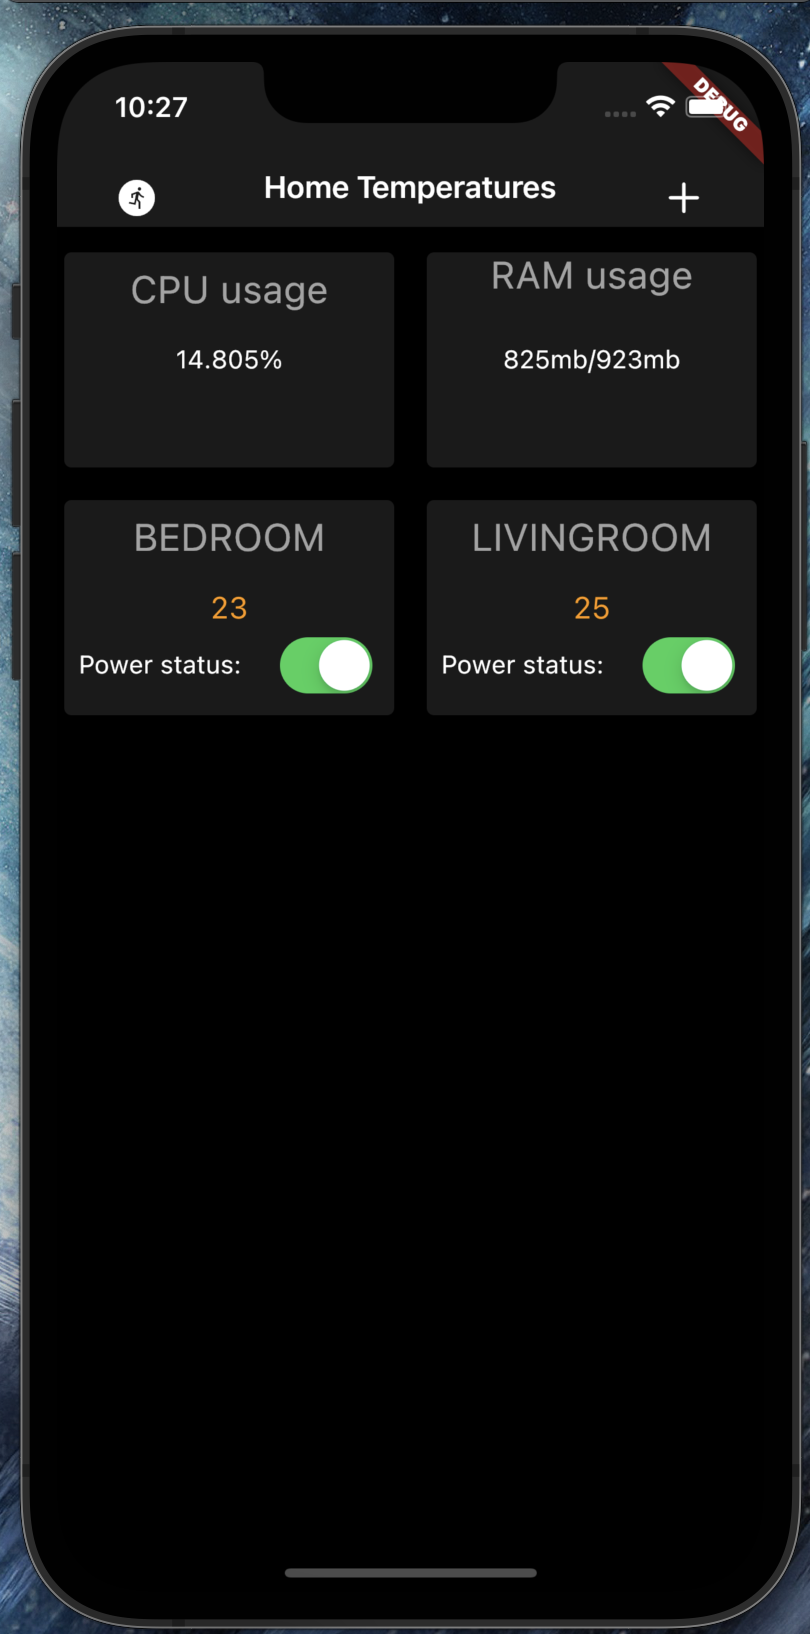
\includegraphics[width=0.5\textwidth]{img/homeScreen.png} 
    \caption{Flutter application main screen}
    \label{fig:appHome}
\end{figure}

\begin{figure}[H]
    \begin{lstlisting}[language=c++]
GestureDetector(
onLongPress: () {
    openDialog(context, i);
},
child: Card(
    color: Colors.white10,
    child: Padding(
    padding: const EdgeInsets.all(8.0),
    child: GridTile(
        header: Text(
        sensorData.sensors[i].Location.toUpperCase(),
        style: const TextStyle(color: Colors.white60),
        textScaleFactor: 1.5,
        textAlign: TextAlign.center,
        ),
        child: GridTileBar(
        subtitle: sensorData.sensors[i].Status
            ? TemperatureText(
                sensorData.sensors[i].Temperature)
            : const Text(
                "Offline",
                textAlign: TextAlign.center,
                ),
        ),
        footer: Row(
        mainAxisAlignment: MainAxisAlignment.spaceBetween,
        children: [
            const Text(
            "Power status: ",
            textScaleFactor: 1,
            style: TextStyle(color: Colors.white),
            ),
            CupertinoSwitch(
            value: sensorData.sensors[i].Status,
            onChanged: (newVal) =>
                sensorData.changePowerStatus(newVal, i),
            ),
        ],
        ),
    ),
    ),
),
);

\end{lstlisting}
    \caption{The Dart code for creating a tile}
    \label{code:app:tile}
\end{figure}

To help with keeping a global state a package\cite{provider} was added. This package enables widgets to listen for changes in class variables and function outputs and then updates the UI accordingly. I used this package to manage a global state of temperature sensors and system usage of the CoAP-server. Whenever new data is available the class calls notifyListeners() functions that tells every listener to update the UI.

To enable the user to add a new temperature sensor a dialog popup was created. The popup requires the user to input a name and the initial power status for the temperature sensor. A dialog in Flutter does not have the same state capabilities as a normal Widget. For user input to be validated state is needed. I solved this by using a special widget called StatefulBuilder. This widget creates its own inner state and instead of taking children it takes a function that returns a widget. Inside this function it has its own state management to re-render the UI as needed. The code for the dialog can be found in figure \ref{code:app:add}

\begin{figure}[H]
    \begin{lstlisting}[language=c++]
StatefulBuilder(
builder: (context, setState) {
    return CupertinoAlertDialog(
    title: const Text("Add sensor"),
    content: Column(
        children: [
        CupertinoTextField(
            placeholder: "location",
            keyboardType: TextInputType.name,
            controller: _locationController,
        ),
        const SizedBox(
            height: 10,
        ),
        Row(
            mainAxisAlignment: MainAxisAlignment.spaceBetween,
            children: [
            const Text(
                "Power status: ",
                textScaleFactor: 1.5,
            ),
            CupertinoSwitch(
                value: initialState,
                onChanged: (val) => setState(
                () {
                    initialState = !initialState;
                },
                ),
            ),
            ],
        ),
        ],
    ),
    actions: [
        CupertinoDialogAction(
        child: const Text("Close"),
        onPressed: () => Navigator.of(context).pop(),
        isDestructiveAction: true,
        ),
        CupertinoDialogAction(
        child: const Text("Add"),
        onPressed: submit,
        ),
    ],
    );
},
);
    \end{lstlisting}
    \caption{The Dart code for creating the add dialog}
    \label{code:app:add}
\end{figure}

The last component to complete the app is the capability to run benchmark. To make it easier to create metrics a package\cite{dartStat} was added. The package can calculated a number of different metrics given an array of data. For this project we are only interested in mean, standard deviation, min and max. 

To get the benchmark results a function is run to calculate the RTT. The app publishes to /all. This publish message is then distributed through the MQTT-broker and picked up by the Translator. The Translator then sends a request to the CoAP-server. When the Translator gets a response from the CoAP-server it the publishes to the MQTT-broker which then distributes the message back to the Flutter application. When the application receives the message it can then derive the round trip time.

To ensure only one message is sent at a time another package\cite{dartMutex} containing mutex locks was added. Even tho Dart is single thread code can still occur asynchronous. Before a new message is sent from the application it needs to acquire the mutex lock. The lock is then released upon receiving the response. This way only one request can be active at a time. The code for the main benchmark function can be found in figure \ref{code:app:bench} and a code snippet showing how the stats package is used can be found in figure \ref{code:app:stat}

\begin{figure}[H]
    \begin{lstlisting}[language=c++]
Future<List<Duration>> benchmark(int runs) async {
    runningBenchmark = true;
    if (bench.isLocked) bench.release();
    b.clear();
    final benchStart = DateTime.now();
    for (var i = 0; i < runs; i++) {
        await bench.acquire();
        print("run: $i");
        lastStartTime = DateTime.now();
        final builder = MqttClientPayloadBuilder();
        builder.addString("GET:$devId");
        client.publishMessage("all", MqttQos.atMostOnce, builder.payload!);
    }
    await bench.acquire();
    runningBenchmark = false;
    totalTime = DateTime.now().difference(benchStart).inMilliseconds;
    bench.release();

    return b;
}
    \end{lstlisting}
    \caption{The Dart code for running the benchmark}
    \label{code:app:bench}
\end{figure}

\begin{figure}[H]
    \begin{lstlisting}[language=c++]
final stat = Stats.fromData(l.map((e) => e.inMilliseconds)
        .toList()).withPrecision(3);
final reqPerSec = l.length /
(Provider.of<SensorProvider>(context, listen: false).totalTime / 1000);
    \end{lstlisting}
    \caption{The Dart code for calculating statistics}
    \label{code:app:stat}
\end{figure}

The benchmark results are displayed in a dialog popup. While the benchmark is running it displays running benchmark otherwise it displays the results. Examples of this can be found in figure \ref{fig:appBenchRun} and figure \ref{fig:appBenchRes} respectively. 

\begin{figure}[H]
    \centering
    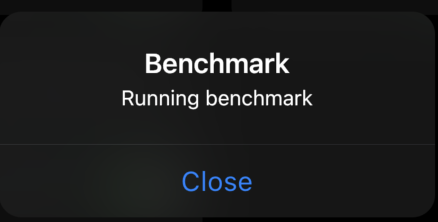
\includegraphics[width=0.7\textwidth]{img/becnhrun.png} 
    \caption{Dialog while benchmark is running}
    \label{fig:appBenchRun}
\end{figure}

\begin{figure}[H]
    \centering
    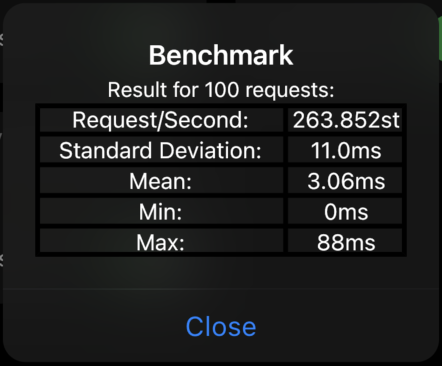
\includegraphics[width=0.7\textwidth]{img/becnhdone.png} 
    \caption{Dialog when benchmark is done}
    \label{fig:appBenchRes}
\end{figure}
